\documentclass[11pt,a4paper]{article}
\usepackage[top=3cm, bottom=2cm, left=2cm, right=2cm]{geometry}
\usepackage[utf8]{inputenc}
\usepackage{amsmath, amsfonts, amssymb}
\usepackage{siunitx}
\usepackage[brazil]{babel}
\usepackage{graphicx}
\usepackage[margin=10pt,font={small, it},labelfont=bf, textfont=it]{caption}
\usepackage[dvipsnames, svgnames]{xcolor}
\DeclareCaptionFont{MediumOrchid}{\color[svgnames]{MediumOrchid}}
\usepackage[pdftex]{hyperref}
\usepackage{natbib}
\bibliographystyle{plainnat}
\bibpunct{\textcolor{MediumOrchid}{\textbf{[}}}{\textcolor{MediumOrchid}{\textbf{]}}}{,}{s}{}{}
\usepackage{color}
\usepackage{footnote}
\usepackage{setspace}
\usepackage{booktabs}
\usepackage{multirow}
\usepackage{subfigure}
\usepackage{fancyhdr}
\usepackage{leading}
\usepackage{indentfirst}
\usepackage{wrapfig}
\usepackage{mdframed}
\usepackage{etoolbox}
\usepackage[version=4]{mhchem}
\usepackage{enumitem}
\usepackage{caption}
\usepackage{titlesec}
\usepackage{tcolorbox}
\usepackage{tikz}
\usepackage{LobsterTwo}
\usepackage[T1]{fontenc}
\usepackage{fontspec}
\usepackage{txfonts}
\usepackage[bottom]{footmisc}
\tcbuselibrary{skins,breakable}
\sisetup{output-decimal-marker={.}}

\makeatletter
\def\footnoterule{\kern-3pt\color{MediumOrchid}\hrule\@width0.6\textwidth height 0.8pt\kern2.6pt}
\makeatother

\renewcommand{\footnotelayout}{\itshape\color{MediumOrchid}}

\AtBeginEnvironment{equation}{\fontsize{13}{16}\selectfont}


\titleformat{\section}{\LobsterTwo\LARGE\color{CarnationPink}}{\thesection.}{1em}{}
\titleformat{\subsection}{\LobsterTwo\LARGE\color{CarnationPink}}{\thesubsection}{1em}{}
\titleformat{\subsubsection}{\LobsterTwo\large\color{CarnationPink}}{\thesubsubsection}{1em}{}


\DeclareCaptionLabelFormat{figuras}{\textcolor{DarkTurquoise}{Figura \arabic{figure}}}
\captionsetup[figure]{labelformat=figuras}

\makeatletter
\renewcommand\tagform@[1]{\maketag@@@{\color{CarnationPink}(#1)}}
\makeatother

\renewcommand{\theequation}{Eq. \arabic{equation}}
\renewcommand{\thefigure}{Fig. \arabic{figure}}
\renewcommand{\thesection}{\textcolor{CarnationPink}{\arabic{section}}}

\setlist[itemize]{label=\textcolor{CarnationPink}{$\blacksquare$}}

\setlist[enumerate]{label=\textcolor{CarnationPink}{\arabic*.}, align=left, leftmargin=1.5cm}


\newcounter{exemplo}

\NewDocumentEnvironment{exemplo}{ O{} }{%
\allowbreak
\setlength{\parindent}{0pt}
  \begin{mdframed}[
  leftline=true,
  topline=false,
  rightline=false,
  bottomline=false,
  linewidth=2pt,
  linecolor=CarnationPink,
  frametitlerule=false,
  frametitlefont=\LobsterTwo\large\color{CarnationPink},
  frametitle={\color{CarnationPink}\LobsterTwo\large #1},
  ]
}{%
  \end{mdframed}
}

\setlength{\fboxsep}{5pt}
\setlength{\fboxrule}{1.5pt}
\usepackage{float}
\renewcommand{\thefootnote}{\alph{footnote}}
\usepackage{url}
\hypersetup{
	colorlinks=true,
	linkcolor=DarkTurquoise,
	filecolor=DarkTurquoise,      
	urlcolor=DarkTurquoise,
	citecolor=DarkTurquoise,
	pdftitle={Especialista em Física da Radioterapia}
}
\pagestyle{fancy}
\fancyhf{}
\renewcommand{\headrulewidth}{0pt}
\rfoot{Página \thepage}

\title{\LobsterTwo\Huge{Radiobiologia}}
\author{\LobsterTwo\Large{Razão Terapêutica}\nocite{*}}
\date{\LobsterTwo\textit{Dalila Mendonça}}
\begin{document}
	\maketitle

\section{Introdução}

	O objetivo da radioterapia é tratar efetivamente os tumores enquanto se minimiza os danos aos tecidos normais. Modelos preditivos podem ser utilizados para calcular as probabilidades de controle tumoral (TCP) e as probabilidades de complicações nos tecidos normais (NTCP). Aumentar a dose de radiação ou o volume de radiação geralmente leva a valores mais altos de TCP e NTCP. A diferença entre TCP e NTCP é conhecida como janela terapêutica. No entanto, certos fatores, como erro geográfico e repopulação acelerada, podem diminuir o TCP e, consequentemente, estreitar a janela terapêutica. A combinação da radioterapia com outras modalidades de tratamento, como quimioterapia e imunoterapia, pode potencialmente modificar a janela terapêutica.

\section{Curvas de Probabilidade de Controle Tumoral (TCP)}

	As curvas de Probabilidade de Controle Tumoral (TCP) são ferramentas utilizadas na radioterapia para estimar a probabilidade de um tumor ser controlado em função da dose total de radiação administrada. Essas curvas são geradas ao plotar a probabilidade de controle tumoral em relação à dose de radiação.

	Existem diferentes maneiras de construir as curvas de TCP. Elas podem ser baseadas em dados clínicos de pacientes tratados, em experimentos laboratoriais ou em modelos teóricos. Mesmo quando se utiliza dados clínicos, é necessário um modelo teórico para descrever a resposta das células tumorais à radiação. Esses modelos levam em consideração fatores como a radiossensibilidade do tumor, a capacidade de reparo do DNA e a proliferação celular.

	As curvas de TCP geralmente têm uma forma sigmoidal, exibindo uma resposta mínima em doses muito baixas, um aumento gradual da probabilidade de controle tumoral na faixa de doses intermediárias e um platô em doses mais altas. Isso significa que o aumento da dose de radiação resulta em um aumento gradual na probabilidade de controle do tumor, mas em doses mais altas, há um limite além do qual aumentos adicionais na dose têm pouco impacto no controle tumoral.

	Essas curvas são de grande importância na prática clínica, pois fornecem informações valiosas para os radioterapeutas na seleção da dose de radiação a ser administrada. Elas auxiliam na busca de um equilíbrio entre a probabilidade de controle tumoral e a minimização dos efeitos colaterais nos tecidos normais circundantes. As curvas de TCP ajudam os profissionais de radioterapia a tomar decisões personalizadas sobre o planejamento do tratamento, levando em consideração as características do tumor e do paciente, para maximizar os resultados terapêuticos.

\subsection*{Cálculo da Probabilidade de Controle Tumoral (TCP)}

	A probabilidade de controle tumoral (TCP) é calculada com base na suposição de que uma única célula tumoral clonogênica é capaz de iniciar o crescimento de um tumor completo. A TCP representa a probabilidade de que nenhuma célula tumoral clonogênica sobreviva ao tratamento.

	Usando estatísticas de Poisson, se houver uma média de $X$ células tumorais clonogênicas, a TCP pode ser calculada como $e^{-X}$, onde $e$ é o número de Euler ($2,71828...$). Em outras palavras, a TCP é igual ao exponencial negativo do número médio de células tumorais clonogênicas.

	Uma abordagem prática é estabelecer uma taxa de sobrevida das células tumorais desejada ($1 - \text{TCP}$). Por exemplo, se o objetivo é alcançar uma TCP de 90\%, a taxa de sobrevida das células tumorais seria de 0.1 ($1 - 0.9$).

	\begin{tcolorbox}[width=\textwidth, colback={white}, colbacktitle={DarkTurquoise!50!white}, title={$\bigstar$ \LobsterTwo{Para Entender Melhor} $\bigstar$}, coltitle={CarnationPink}, colframe={DarkTurquoise}, fonttitle=\rmfamily\bfseries\Large, breakable]

		Para ilustrar a situação onde, para  alcançar uma TCP de 90\%, a taxa de sobrevida das células tumorais dever ser de 0.1:
		
		\begin{itemize}[label=\textcolor{CarnationPink}{$\blacktriangleright$}]
			\item Se o número inicial de células tumorais clonogênicas for de $10^9$, a fração de sobrevivência desejada seria de $10^{-10}$ para alcançar uma TCP de 90\%. 
				\begin{itemize}[label=\textcolor{CarnationPink}{$\star$}]
					\item Isso significa que, para alcançar uma TCP de 90\% para cada $10^9$ células tumorais clonogênicas iniciais, espera-se que apenas 0.1 em cada $10^{9}$ células sobreviva ao tratamento.
				\end{itemize}
			\end{itemize}
	\end{tcolorbox}


\subsection*{Fatores que Afetam a Forma e a Inclinação das Curvas de TCP}

	A inclinação ($\gamma$) de uma curva de probabilidade de controle tumoral (TCP) representa a relação entre a mudança absoluta na probabilidade de resposta e a mudança relativa na dose. Por exemplo, um valor de $\gamma$ igual a 2 indica que um aumento de 1\% na dose resulta em um aumento de 2\% na TCP. A inclinação varia ao longo da curva de TCP, sendo maior na faixa de doses intermediárias, o que significa que pequenas mudanças na dose nessa região têm um impacto maior na probabilidade de controle tumoral. Em contraste, em doses muito baixas e muito altas, a resposta à dose é mais suave, com uma inclinação menor ($\gamma$ baixo) (\ref{fig:CurvaTcp}).

	\begin{figure}[h]
		\centering
		\fcolorbox{DarkTurquoise}{white}{%
			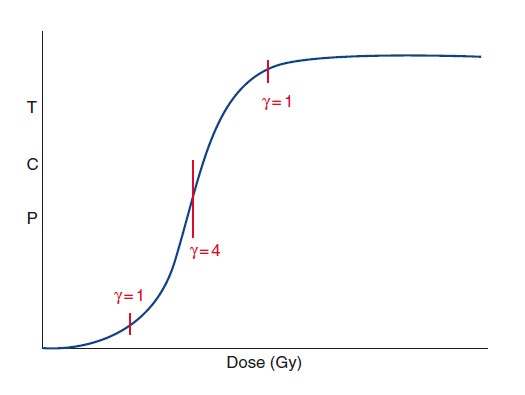
\includegraphics[width=0.5\textwidth]{Imagens/CurvaTcp.jpg}
		}%
		\caption{Curva TCP mostrando vários valores de $\gamma$.}
		\label{fig:CurvaTcp}
	\end{figure}

	O método de administração da dose também pode influenciar a inclinação da curva de TCP. Quando o escalonamento da dose é alcançado por meio de mais frações com tamanho de fração fixo, a inclinação medida será menor em comparação com o escalonamento da dose através do aumento do tamanho da fração. Isso ocorre porque, ao aumentar o tamanho da fração, as mudanças absolutas na dose têm um impacto maior na TCP, resultando em uma inclinação maior da curva (\ref{fig:curvaTcpDiferentesResistencias}).

	\begin{figure}[h]
		\centering
		\fcolorbox{DarkTurquoise}{white}{%
			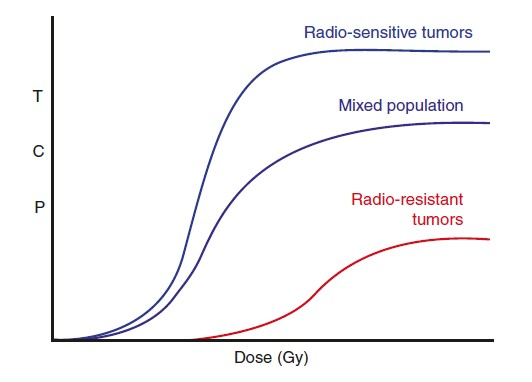
\includegraphics[width=0.5\textwidth]{Imagens/curvaTcpDiferentesResistencias.jpg}
		}%
		\caption{.}
		\label{fig:curvaTcpDiferentesResistencias}
	\end{figure}

	A presença de uma população mista de tumores pode afetar a resposta à dose, resultando em uma inclinação mais suave da curva de TCP. Isso ocorre porque tumores muito sensíveis podem ser controlados mesmo em níveis de dose mais baixos, enquanto tumores mais resistentes podem permanecer descontrolados mesmo em níveis de dose mais altos. A presença de uma população mista dilui a resposta à dose em comparação com uma população homogênea de tumores.

	Além disso, a falha em abranger toda a região tumoral, conhecida como "geographic miss", torna-se mais significativa à medida que a TCP se aproxima de níveis elevados. Mesmo com o escalonamento da dose, se houver células tumorais fora do campo de radiação, essas células não serão controladas, independentemente da dose administrada. Portanto, é crucial garantir uma cobertura adequada de todo o tumor-alvo para maximizar a probabilidade de controle tumoral.

\section{Probabilidade de Complicação de Tecido Normal (NTCP)}


	A probabilidade de complicação do tecido normal (NTCP) é uma medida da probabilidade de ocorrência de lesões em tecidos normais devido à radiação. Assim como a probabilidade de controle tumoral (TCP), a NTCP é construída plotando a probabilidade de lesão do tecido normal em função da dose de radiação recebida.

	Em comparação aos tumores, o tecido normal geralmente apresenta uma relação dose-resposta mais íngreme. Isso significa que mesmo pequenos aumentos na dose de radiação podem resultar em um aumento significativo na probabilidade de complicações no tecido normal.

	A dependência do volume irradiado é um aspecto importante na NTCP. O modelo LKB (\textit{Lyman-Kutcher-Burman}) incorpora essa dependência introduzindo um expoente de volume, denotado como "n". Tecidos com um grande efeito de volume, chamados de tecidos paralelos, têm um valor maior de "n". Por outro lado, tecidos com um pequeno efeito de volume, conhecidos como tecidos seriais, têm um valor menor de "n". Essa relação é uma tentativa de capturar a variação da resposta do tecido normal em diferentes volumes irradiados.

	É essencial observar que, na prática clínica, os órgãos normais raramente são irradiados de forma uniforme. Portanto, é necessário levar em consideração os volumes variáveis de irradiação que diferentes órgãos podem receber. O modelo LKB utiliza um histograma dose-volume (DVH) para calcular uma dose e um volume equivalentes, assumindo irradiação uniforme em uma parte do órgão. No entanto, é importante interpretar os resultados dessas análises com cautela, pois o modelo LKB é uma aproximação matemática e não possui uma base biológica sólida que explique completamente as complexidades dos efeitos da radiação no tecido normal.

\section{Janela Terapêutica e Razão Terapêutica}


	A janela terapêutica na radioterapia é um conceito fundamental que busca encontrar um equilíbrio entre o controle do tumor e a toxicidade nos tecidos normais. Ela representa a faixa de doses ou estratégias de tratamento em que é possível alcançar o controle efetivo do tumor, ao mesmo tempo em que se minimiza os danos aos tecidos saudáveis circundantes. Embora a janela terapêutica não possa ser quantificada com um valor específico, ela é uma medida relativa da segurança e eficácia do tratamento. Quanto maior a janela terapêutica, maior a probabilidade de obter resultados favoráveis no tratamento (\ref{fig:TcpENtcp}).

	\begin{figure}[h]
		\centering
		\fcolorbox{DarkTurquoise}{white}{%
			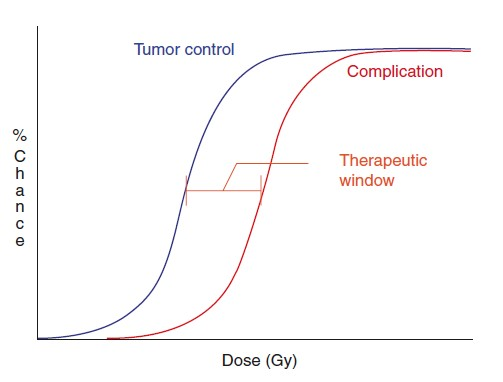
\includegraphics[width=0.5\textwidth]{Imagens/TcpENtcp.jpg}
		}%
		\caption{A janela terapêutica é a diferença entre a curva TCP e a curva NTCP.}
		\label{fig:TcpENtcp}
	\end{figure}

	A razão terapêutica é uma medida que nos permite avaliar a relação benefício-risco do tratamento radioterápico. Ela é calculada levando em consideração a probabilidade de controle do tumor (TCP) e a probabilidade de complicação do tecido normal (NTCP). A equação comumente usada para calcular a razão terapêutica é 
	
	\begin{equation}
		\text{RT} = \text{TCP} \times (1 - \text{NTCP})
	\end{equation}
	
	Multiplicando a probabilidade de controle do tumor pela probabilidade complementar de complicação do tecido normal, obtemos uma medida que reflete a diferença entre o controle do tumor e a toxicidade nos tecidos normais. No entanto, é importante destacar que a aplicação prática dessa equação requer a obtenção de valores confiáveis e precisos para a TCP e NTCP, que são estimados com base em dados clínicos, experimentais e modelos matemáticos.

	A seleção de uma técnica de entrega de dose de radiação ideal para o tratamento de um tumor específico visa maximizar a probabilidade de controle do tumor (TCP), ao mesmo tempo em que minimiza a probabilidade de complicações nos tecidos normais (NTCP). Em um tratamento efetivo de radioterapia típico, os objetivos desejados são TCP $\geq$ 0.5 (indicando uma alta probabilidade de controle do tumor) e NTCP $\leq$ 0.05 (indicando uma baixa probabilidade de complicações nos tecidos normais). 

	É importante destacar que existem diferentes formas de definir a razão terapêutica, e a equação apresentada é apenas uma delas. Dependendo do contexto específico, outras definições podem ser utilizadas. Além disso, a escolha da definição de "complicação" pode variar e influenciar a razão terapêutica. Em algumas situações clínicas, os pacientes podem experimentar diferentes níveis de toxicidade, especialmente em áreas sensíveis como a cabeça e o pescoço. Portanto, é essencial determinar qual nível de toxicidade é considerado aceitável ou inaceitável, levando em consideração os riscos e benefícios do tratamento, ao avaliar a razão terapêutica.

	Ao considerar a razão terapêutica, é essencial ter em mente que ela não é uma medida absoluta, mas sim uma ferramenta de avaliação que auxilia na tomada de decisões clínicas. A interpretação e análise cuidadosa da razão terapêutica, levando em consideração as características individuais do paciente, os objetivos de tratamento e os riscos envolvidos, são cruciais para garantir a melhor abordagem terapêutica e maximizar os benefícios para o paciente.
		
\subsection*{Repopulação do Tecido Normal e Tumoral}

	Durante o tratamento prolongado por radiação, tanto os tumores quanto os tecidos normais têm o potencial de passar por repopulação celular (\ref{fig:repopulacaoAcelerada}). O repopulação refere-se ao aumento do número de células após a morte inicial das células induzida pela radiação. No entanto, é importante observar que os tumores tendem a se repovoar de forma mais eficiente do que os tecidos normais. Isso ocorre porque as células tumorais muitas vezes têm uma taxa de proliferação mais alta e uma capacidade de recuperação mais rápida em comparação com as células normais.

	\begin{figure}[h]
		\centering
		\fcolorbox{DarkTurquoise}{white}{%
			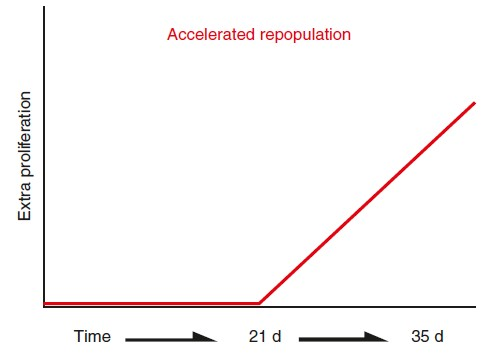
\includegraphics[width=0.5\textwidth]{Imagens/repopulacaoAcelerada.jpg}
		}%
		\caption{Alguns tumores passam por um repovoamento acelerado após um determinado período de tratamento. Isso é conhecido como tempo de início (kickoff time). Esse efeito pode frequentemente diminuir a janela terapêutica.}
		\label{fig:repopulacaoAcelerada}
	\end{figure}

	O repopulação das células tumorais tem implicações na radioterapia, especialmente em relação à probabilidade desejada de controle tumoral (TCP). O aumento da proliferação celular nos tumores pode exigir doses de radiação mais altas para alcançar o mesmo nível de controle tumoral que seria obtido em um cenário de repopulação celular limitada. Isso é visualizado pela curva de TCP, que se desloca para a direita, indicando a necessidade de doses mais altas para manter a eficácia do tratamento (\ref{fig:tcpNtcpEQT}).

	\begin{figure}[h]
		\centering
		\fcolorbox{DarkTurquoise}{white}{%
			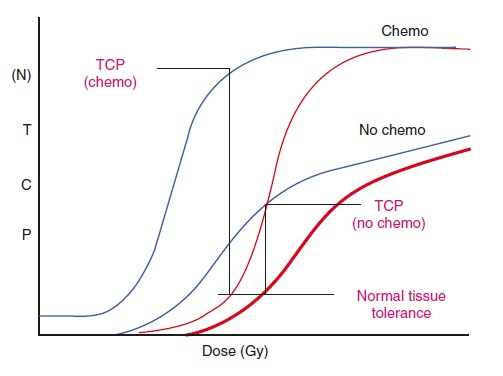
\includegraphics[width=0.5\textwidth]{Imagens/tcpNtcpEQT.jpg}
		}%
		\caption{Curvas de TCP (azul) e curvas de NTCP (vermelho) mostrando o efeito da quimioterapia radiosensibilizante (deslocada para a esquerda) em comparação com a ausência de quimioterapia (deslocada para a direita).}
		\label{fig:tcpNtcpEQT}
	\end{figure}

	Da mesma forma, o repopulação dos tecidos normais pode aumentar a probabilidade de complicações nos tecidos saudáveis adjacentes ao tumor, como os tecidos normais respondem de maneira menos eficiente ao dano causado pela radiação. O aumento da proliferação celular nos tecidos normais resulta em uma curva de NTCP deslocada para a direita, indicando um aumento na probabilidade de toxicidade nos tecidos normais adjacentes.

	No entanto, é importante destacar que os tecidos normais que respondem tardiamente, como o tecido normal do sistema nervoso central, têm uma capacidade de repopulação limitada em escalas de tempo clinicamente relevantes. Isso significa que sua capacidade de regeneração e recuperação dos danos causados pela radiação é limitada, e o repopulação não é o principal fator que impulsiona os efeitos da prolongação do tratamento nesses tecidos.

	Em geral, a prolongação do tratamento é considerada desfavorável, pois estreita a janela terapêutica, reduzindo a margem entre o controle tumoral e a toxicidade nos tecidos normais. Estudos clínicos em pacientes com cânceres de células escamosas nas regiões da cabeça e pescoço ou cânceres ginecológicos demonstraram que um tempo total de tratamento prolongado pode levar a resultados de sobrevivência reduzidos. Portanto, os esforços são feitos para minimizar a prolongação do tratamento e otimizar os esquemas de tratamento, a fim de manter uma janela terapêutica ideal que equilibre o controle tumoral efetivo e a toxicidade nos tecidos normais. Isso pode ser alcançado por meio da otimização da dose, fracionamento e programação do tratamento, bem como pelo uso de técnicas avançadas de radioterapia, como a radioterapia de intensidade modulada (IMRT) e a radioterapia estereotáxica (SRT/SBRT).

\subsection*{Sensibilizadores, Protetores e Modalidade Combinada}

	O objetivo da terapia de modalidade combinada é melhorar a relação terapêutica, que é o equilíbrio entre o controle do tumor e a toxicidade nos tecidos normais. Vários mecanismos podem ser empregados para melhorar essa relação terapêutica:

	\begin{itemize}[label=\textcolor{CarnationPink}{$\blacktriangleright$}]
		\item \textcolor{DarkTurquoise}{\textbf{Sensibilização Seletiva do Tumor:}} 
		
		A sensibilização seletiva do tumor é uma estratégia que visa aumentar a sensibilidade das células tumorais à radiação. Sensibilizadores podem ser agentes químicos, como radiosensibilizadores, que tornam as células tumorais mais suscetíveis aos efeitos da radiação. Eles podem atuar direcionando mecanismos específicos nas células tumorais, aumentando a resposta à radiação e melhorando a eficácia do tratamento.

		\item \textcolor{DarkTurquoise}{\textbf{Proteção Seletiva dos Tecidos Normais:}} 
		
		A proteção seletiva dos tecidos normais busca reduzir a toxicidade nos tecidos saudáveis durante o tratamento de radiação. Isso pode ser alcançado por meio do uso de protetores, como agentes radioprotetores, que ajudam a minimizar os efeitos prejudiciais da radiação nos tecidos normais. Esses protetores podem atuar como antioxidantes ou por outros mecanismos, reduzindo assim a toxicidade nos tecidos normais e preservando sua função.

		\item \textcolor{DarkTurquoise}{\textbf{Eliminação Independente do Tumor:}}
		
		A combinação de diferentes modalidades de tratamento, como radioterapia e quimioterapia, pode resultar em uma eliminação mais eficaz das células tumorais. Isso ocorre porque diferentes modalidades podem agir em mecanismos distintos, direcionando e eliminando as células tumorais de forma independente. A combinação sinérgica dessas modalidades pode melhorar os resultados do tratamento, aumentando a probabilidade de controle tumoral.

		\item \textcolor{DarkTurquoise}{\textbf{Eliminação Seletiva de Tumores Radioresistentes:}}
		
		Em alguns casos, certas células tumorais podem ser mais resistentes à radioterapia, como as células hipóxicas. Estratégias específicas podem ser empregadas para direcionar e eliminar essas células radioresistentes, aumentando assim a eficácia do tratamento. Isso pode envolver o uso de técnicas de hiperoxigenação tumoral, que aumentam a disponibilidade de oxigênio nas células tumorais e as tornam mais suscetíveis à radiação.

		\item \textcolor{DarkTurquoise}{\textbf{Redistribuição de Células Tumorais:}}
		
		A redistribuição de células tumorais é outra estratégia utilizada na terapia de modalidade combinada. Manipular o ciclo celular das células tumorais pode aumentar sua sensibilidade à radiação. Por exemplo, induzir a redistribuição das células tumorais para fases mais sensíveis à radiação, como a fase G2/M do ciclo celular, pode aumentar a eficácia da radioterapia.

		\item \textcolor{DarkTurquoise}{\textbf{Imunoterapia: }}  
		
		A imunoterapia é uma abordagem promissora que tem sido cada vez mais integrada à radioterapia. Ela visa ativar e fortalecer a resposta imunológica do organismo contra os tumores. A imunoterapia pode complementar a radioterapia, melhorando os resultados do tratamento e aumentando o controle tumoral.

	\end{itemize}

	É importante observar que a terapia de modalidade combinada pode ou não resultar em uma melhoria geral da relação terapêutica. Por exemplo, a administração simultânea de cisplatina com irradiação de cabeça e pescoço pode aumentar tanto as taxas de cura quanto a toxicidade. A avaliação da relação terapêutica depende da importância relativa atribuída à toxicidade e aos resultados de cura.




\bibliography{ref.bib}
\end{document}